\documentclass{standalone}
\usepackage{tikz}

\begin{document}
  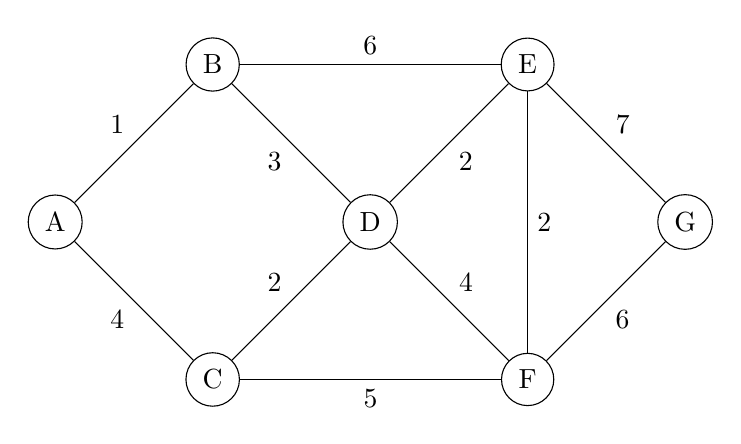
\begin{tikzpicture}
    \node[shape=circle,draw=black] (A) at (-4,0) {A};
    \node[shape=circle,draw=black] (B) at (-2,2) {B};
    \node[shape=circle,draw=black] (C) at (-2,-2) {C};
    \node[shape=circle,draw=black] (D) at (0,0) {D};
    \node[shape=circle,draw=black] (E) at (2,2) {E};
    \node[shape=circle,draw=black] (F) at (2,-2) {F};
    \node[shape=circle,draw=black] (G) at (4,0) {G};

    \path (A) edge node [above left] {1} (B);
    \path (A) edge node [below left] {4} (C);
    \path (B) edge node [below left] {3} (D);
    \path (B) edge node [above] {6} (E);
    \path (C) edge node [above left] {2} (D);
    \path (C) edge node [below] {5} (F);
    \path (D) edge node [below right] {2} (E);
    \path (D) edge node [above right] {4} (F);
    \path (E) edge node [right] {2} (F);
    \path (E) edge node [above right] {7} (G);
    \path (F) edge node [below right] {6} (G);
  \end{tikzpicture}
\end{document}
